\documentclass[12pt, a4]{article}
\usepackage[english]{babel}
\usepackage[utf8]{inputenc}
\usepackage{fullpage}
\usepackage{listings}
\usepackage{graphicx}
\usepackage{color}

%Syntax highlighting
\definecolor{blue-violet}{rgb}{0.54, 0.17, 0.89}
\definecolor{ao}{rgb}{0.0, 0.5, 0.0}
\definecolor{amaranth}{rgb}{0.9, 0.17, 0.31}
\definecolor{ballblue}{rgb}{0.13, 0.67, 0.8}
\definecolor{onyx}{rgb}{0.06, 0.06, 0.06}


\lstset{
  breaklines=true,                 % automatic line breaking only at whitespace
  captionpos=b,                    % sets the caption-position to bottom
  breakatwhitespace=false,
  keepspaces=true,
  numbers=left,
  numbersep=5pt,
  showspaces=false,
  showstringspaces=false,
  showtabs=false,
  tabsize=4,  
  backgroundcolor=\color{white},   % choose the background color
  commentstyle=\color{ao},    % comment style
  keywordstyle=\color{amaranth},    % keyword style
  stringstyle=\color{blue-violet},    % string literal style
  numberstyle=\tiny\color{ballblue},	   % number style
  basicstyle=\ttfamily\footnotesize\color{onyx} % size of fonts used for the code
}


%Document Header
\title{\textbf{Department of CSE\\SSN College of Engineering}}
\author{\textbf{Vishakan Subramanian - 18 5001 196 - Semester VI}}
\date{02 May 2021}

\begin{document}
\maketitle
\hrule
\section*{\center{UCS 1611 - Internet Programming Lab}}
\hrule
\bigskip

%Assignment Details
\subsection*{\center{\textbf{Exercise 8: Programs using Node.js}}}
\subsection*{\flushleft{Learning Objective:}}
\begin{flushleft}

\begin{enumerate}
\item Write a Node.js program that reads all the greetings from the file
greetings.txt, asks the user "What is your name?", then prints a random
greeting followed by the given name. Make sure to check for the case where
the file doesn’t exist! For example, if the greeting is "Hey", then the program
will print "Hey, Joe" to the console, then pick some other greeting and do the
same until finished. Use Non-blocking I/O.
Home, Committee, Call For Papers, Important Dates, Workshops,
Registration and Contact.
\item Write a Node.js program that reads all the greetings as before. When all the greetings are loaded, it creates a server listening on port number 8080. On
request, it checks for whether there is a name value in the query string. If
there isn’t, the value of query.name will be undefined. In other words, if you access http://localhost:8080/?name=Mike, then your browser should just display something like "Hello, Mike" when the page loads.
\newpage
\item Create a web server using node.js which listens for clients request. Once the client request the server, the server returns a web page which contains a list of books and its details in table format.
\item Create a DB with the following details using MongoDB:
\\Database Name: PatientDetails
\\Table Schema: Name, age, ID, gender, address, marital status, Date of Visit
\\Write a node.js program to do the following operations:
\\Add, Delete, Update, Search.
\end{enumerate}



\end{flushleft}


%Code
\newpage
\subsection*{\flushleft{Code - Console Greetings:}}
\begin{flushleft}
\lstinputlisting[language=Java]{Q1/TerminalGreeting.js}
\end{flushleft}

\newpage
\subsection*{\flushleft{Code - Browser Greetings:}}
\begin{flushleft}
\lstinputlisting[language=Java]{Q2/BrowserGreeting.js}
\end{flushleft}

\newpage
\subsection*{\flushleft{Code - Greetings.txt:}}
\begin{flushleft}
\lstinputlisting[]{Q2/greetings.txt}
\end{flushleft}

\newpage
\subsection*{\flushleft{Code - Books.js:}}
\begin{flushleft}
\lstinputlisting[language=Java]{Q3/Books.js}
\end{flushleft}

\newpage
\subsection*{\flushleft{Code - booklist.html:}}
\begin{flushleft}
\lstinputlisting[language=HTML]{Q3/booklist.html}
\end{flushleft}

\newpage
\subsection*{\flushleft{Code - Mongo.js:}}
\begin{flushleft}
\lstinputlisting[language=Java]{Q4/Mongo.js}
\end{flushleft}

%Output
\newpage
\subsection*{\flushleft{Output - Browser Greeting:}}
\begin{figure}[h]
\centering
\caption{Browser Output: Browser Greeting.}
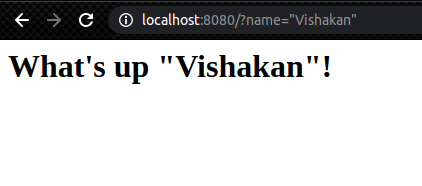
\includegraphics[height=10cm, width=18cm, keepaspectratio]{Output/BrowserGreetingOP.png}
\end{figure}

\newpage
\subsection*{\flushleft{Output - Books Table:}}
\begin{figure}[h]
\centering
\caption{Browser Output: Books Table.}
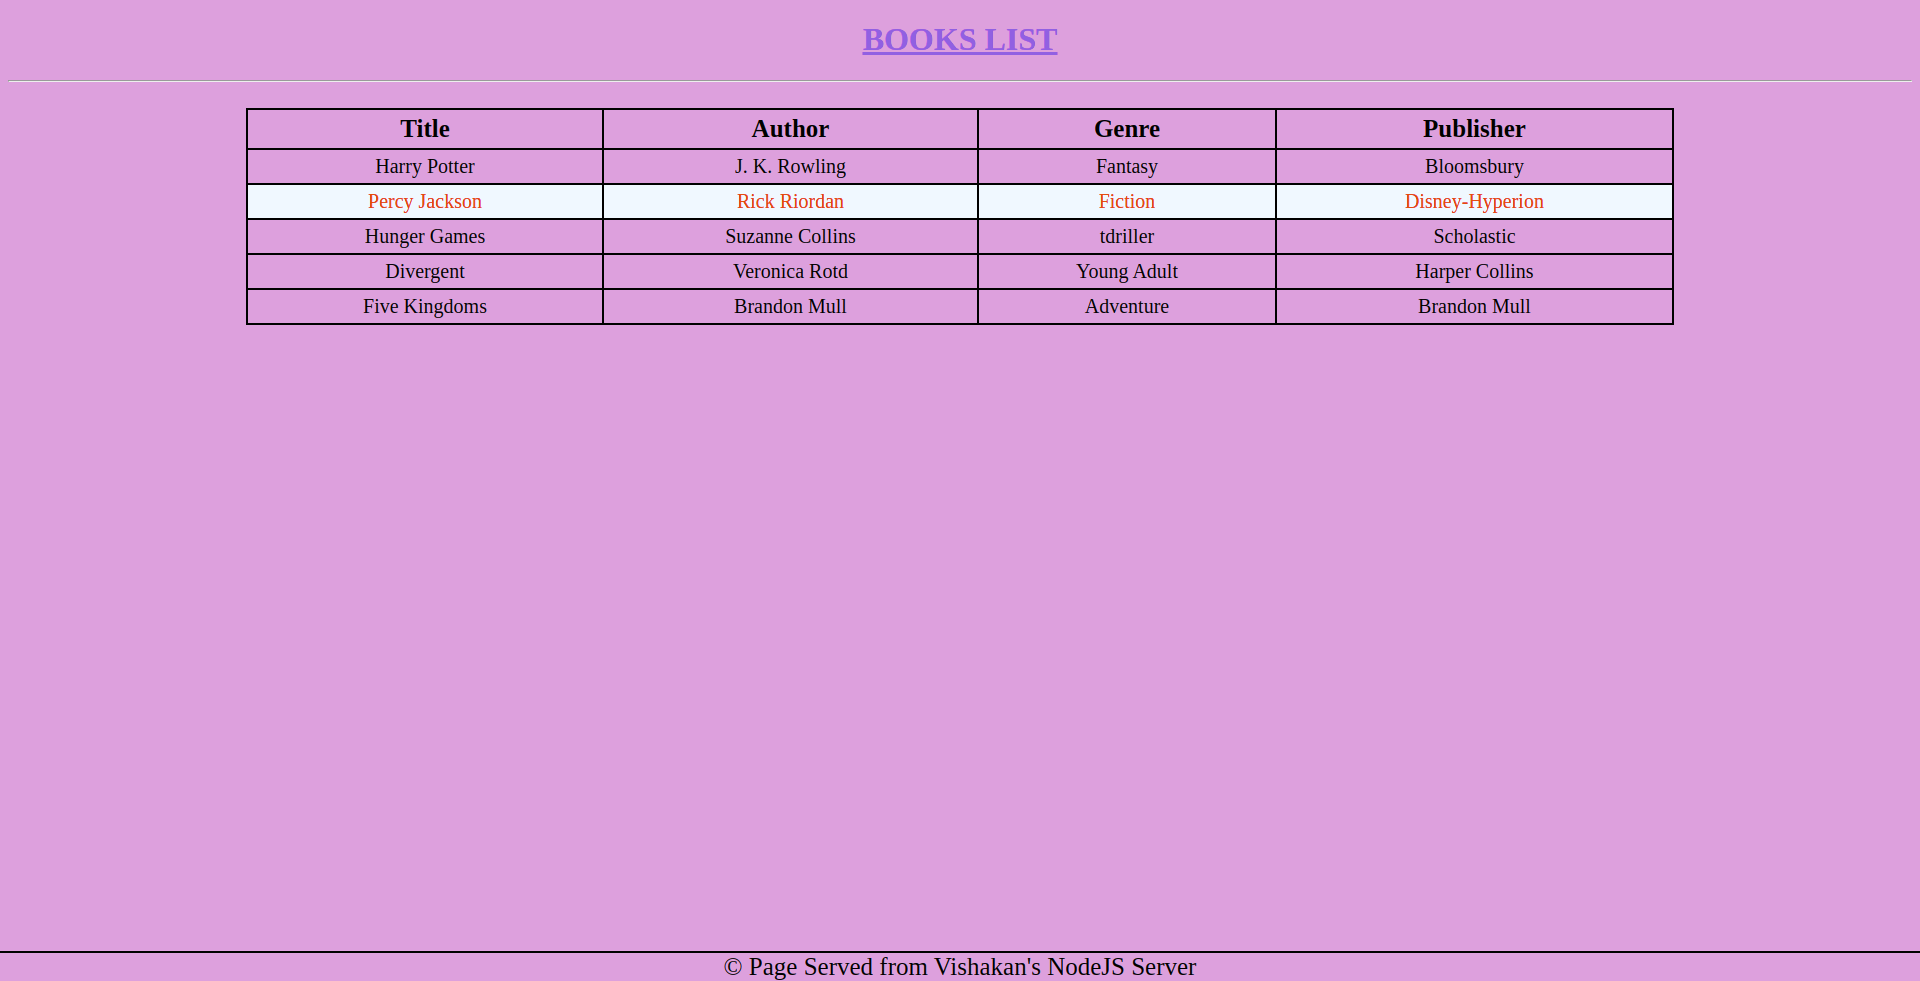
\includegraphics[height=15cm, width=18cm]{Output/BooksOP.png}
\end{figure}

\newpage
\subsection*{\flushleft{Output - Mongo Shell:}}
\begin{figure}[h]
\centering
\caption{Browser Output: Mongo Shell.}
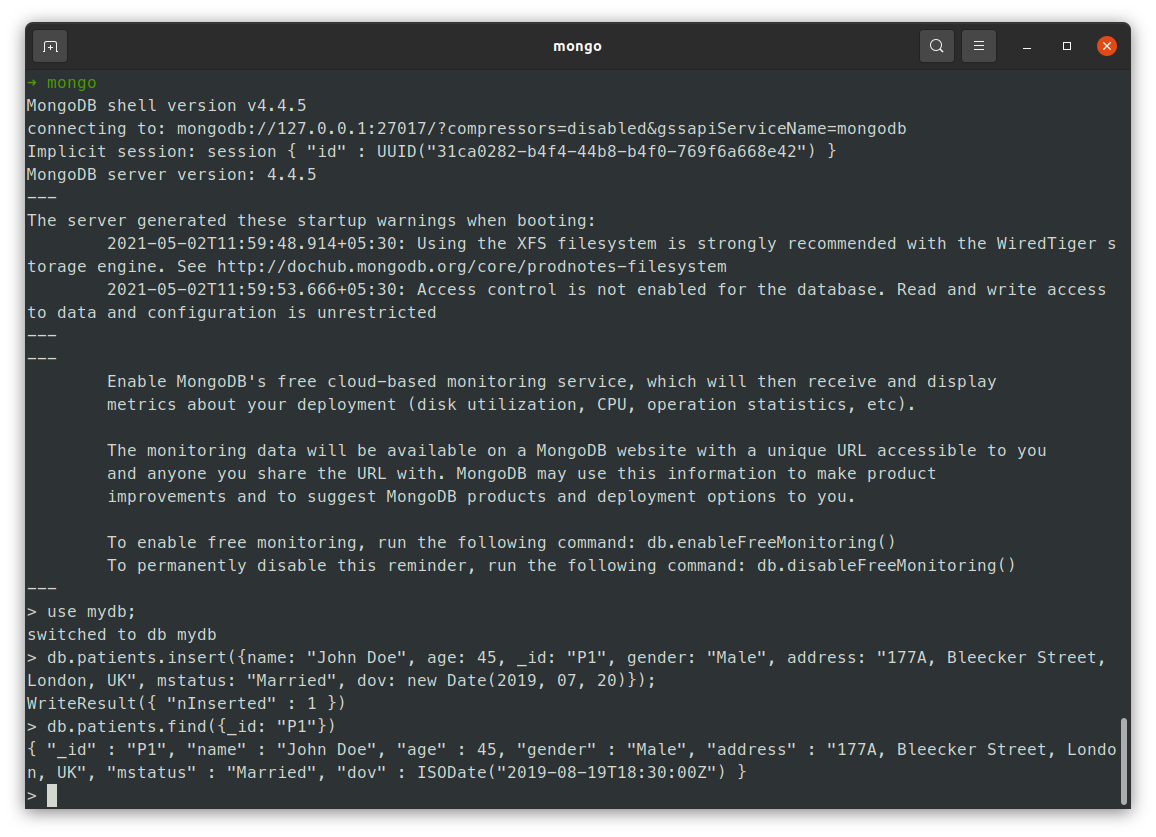
\includegraphics[height=15cm, width=18cm]{Output/MongoOP.png}
\end{figure}

%Learning Outcome
\newpage
\subsection*{\flushleft{Learning Outcome:}}
\begin{itemize}

\item From the experiment, I learnt about NodeJS' event-driven architecture.
\item I learnt to serve HTML content using NodeJS as a server-side application.
\item I learnt to use basic functions available in the \textbf{fs} \& \textbf{http} modules in NodeJS.
\item I learnt to read URL queries and respond to a query with HTML content with \textbf{writeHead() \& write()} methods to serve HTML response.
\item I learnt how to serve a static HTML page using NodeJS to the browser.
\item I installed and learnt to use \textbf{MongoDB} from the shell.
\item I learnt to manipulate a MongoDB database from JavaScript using NodeJS' \textbf{mongodb} module.
\item I understood that these method calls defined by NodeJS for the mongodb moudle are asynchronous, meaning that these operations need not occur one after the other sequentially.
\item Thus, I learnt to implement an \textbf{async-await} methodology to execute the CRUD operations one by one from NodeJS.
\item I was able to successfully perform \textbf{CRUD operations} in MongoDB using NodeJS.
\item I used an \textbf{IIFE}(Immediately Invoked Function Expression) to execute the CRUD driver code.
\item I learnt about MongoDB's syntax and methods like insertOne(), insertMany(), findOne(), deleteOne() and updateOne() to perform CRUD operations.
\item I understood about collections in MongoDB \& the fact that MongoDB is a \textbf{NoSQL} database.
\end{itemize}

\end{document}
